% ==============================================================================
% VISUALISASI GRAFIK STATISTIK
% ==============================================================================

\section*{Visualisasi Grafik Statistik Potensi Wilayah}
\addcontentsline{toc}{section}{Visualisasi Grafik Statistik}

Berikut disajikan visualisasi komparatif dan analisis data potensi statistik 7 wilayah Jaga di Desa Popontolen untuk tahun 2024 dan 2025:

\vspace{0.2cm}

\begin{figure}[!htbp]
  \centering
  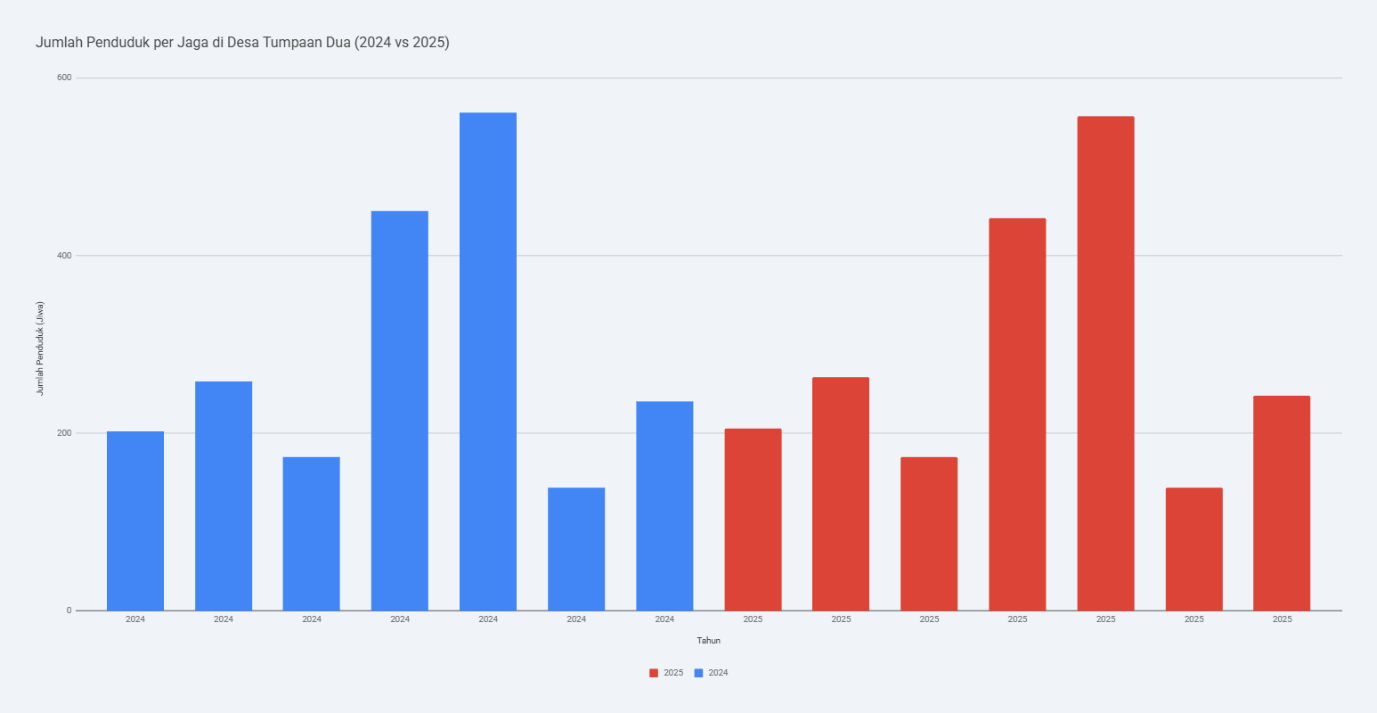
\includegraphics[width=0.85\textwidth]{images/grafik-1-penduduk.png}
  \caption{Jumlah Penduduk per Jaga di Desa Popontolen (Tahun 2024 vs 2025)}
  \label{fig:grafik1}
\end{figure}

\noindent\small Grafik menunjukkan distribusi penduduk yang tidak merata di 7 wilayah Jaga. \textbf{Jaga 7} mendominasi dengan 488 jiwa (31,1\% dari total populasi desa), jauh melampaui jaga lainnya. Terjadi sedikit penurunan populasi dari 1.621 jiwa (2024) menjadi 1.570 jiwa (2025) atau turun 3,1\%, dengan penurunan terbesar di Jaga 4 (dari 237 menjadi 207 jiwa). Konsentrasi penduduk di Jaga 7 menjadi prioritas utama dalam pemerataan alokasi anggaran dan fasilitas publik desa.

\vspace{0.4cm}

\begin{figure}[!htbp]
  \centering
  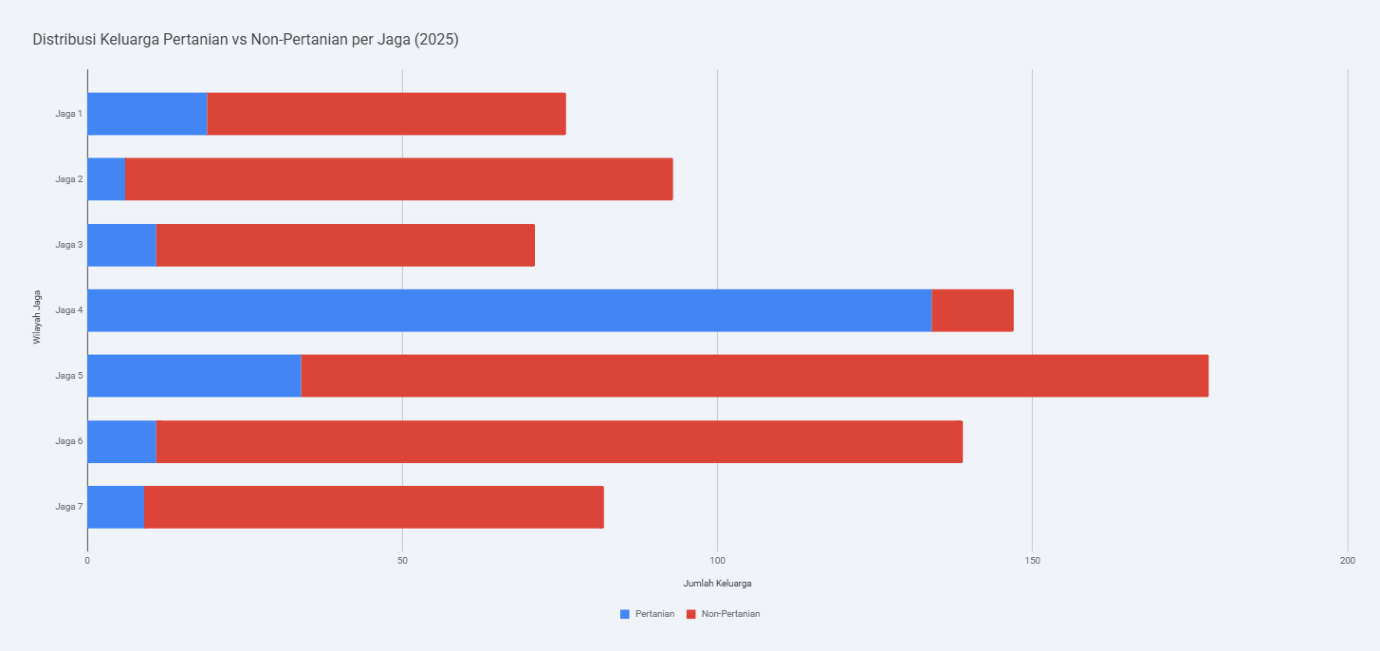
\includegraphics[width=0.85\textwidth]{images/grafik-2-pekerjaan.png}
  \caption{Distribusi Keluarga Pertanian vs Non-Pertanian per Jaga (Tahun 2025)}
  \label{fig:grafik2}
\end{figure}

\noindent\small Sektor non-pertanian mendominasi mata pencaharian warga dengan 272 KK (51,0\%), sementara sektor pertanian menopang 179 KK (33,6\%). \textbf{Jaga 7} memiliki konsentrasi petani tertinggi (67 KK), disusul Jaga 6 (30 KK) dan Jaga 2 (27 KK). Anomali tercatat di Jaga 5 yang seluruh 56 keluarganya belum terdata pada sektor non-pertanian formal, mengindikasikan pola mata pencaharian serabutan atau campuran yang memerlukan pembinaan kelembagaan ekonomi desa.

\clearpage

\begin{figure}[!htbp]
  \centering
  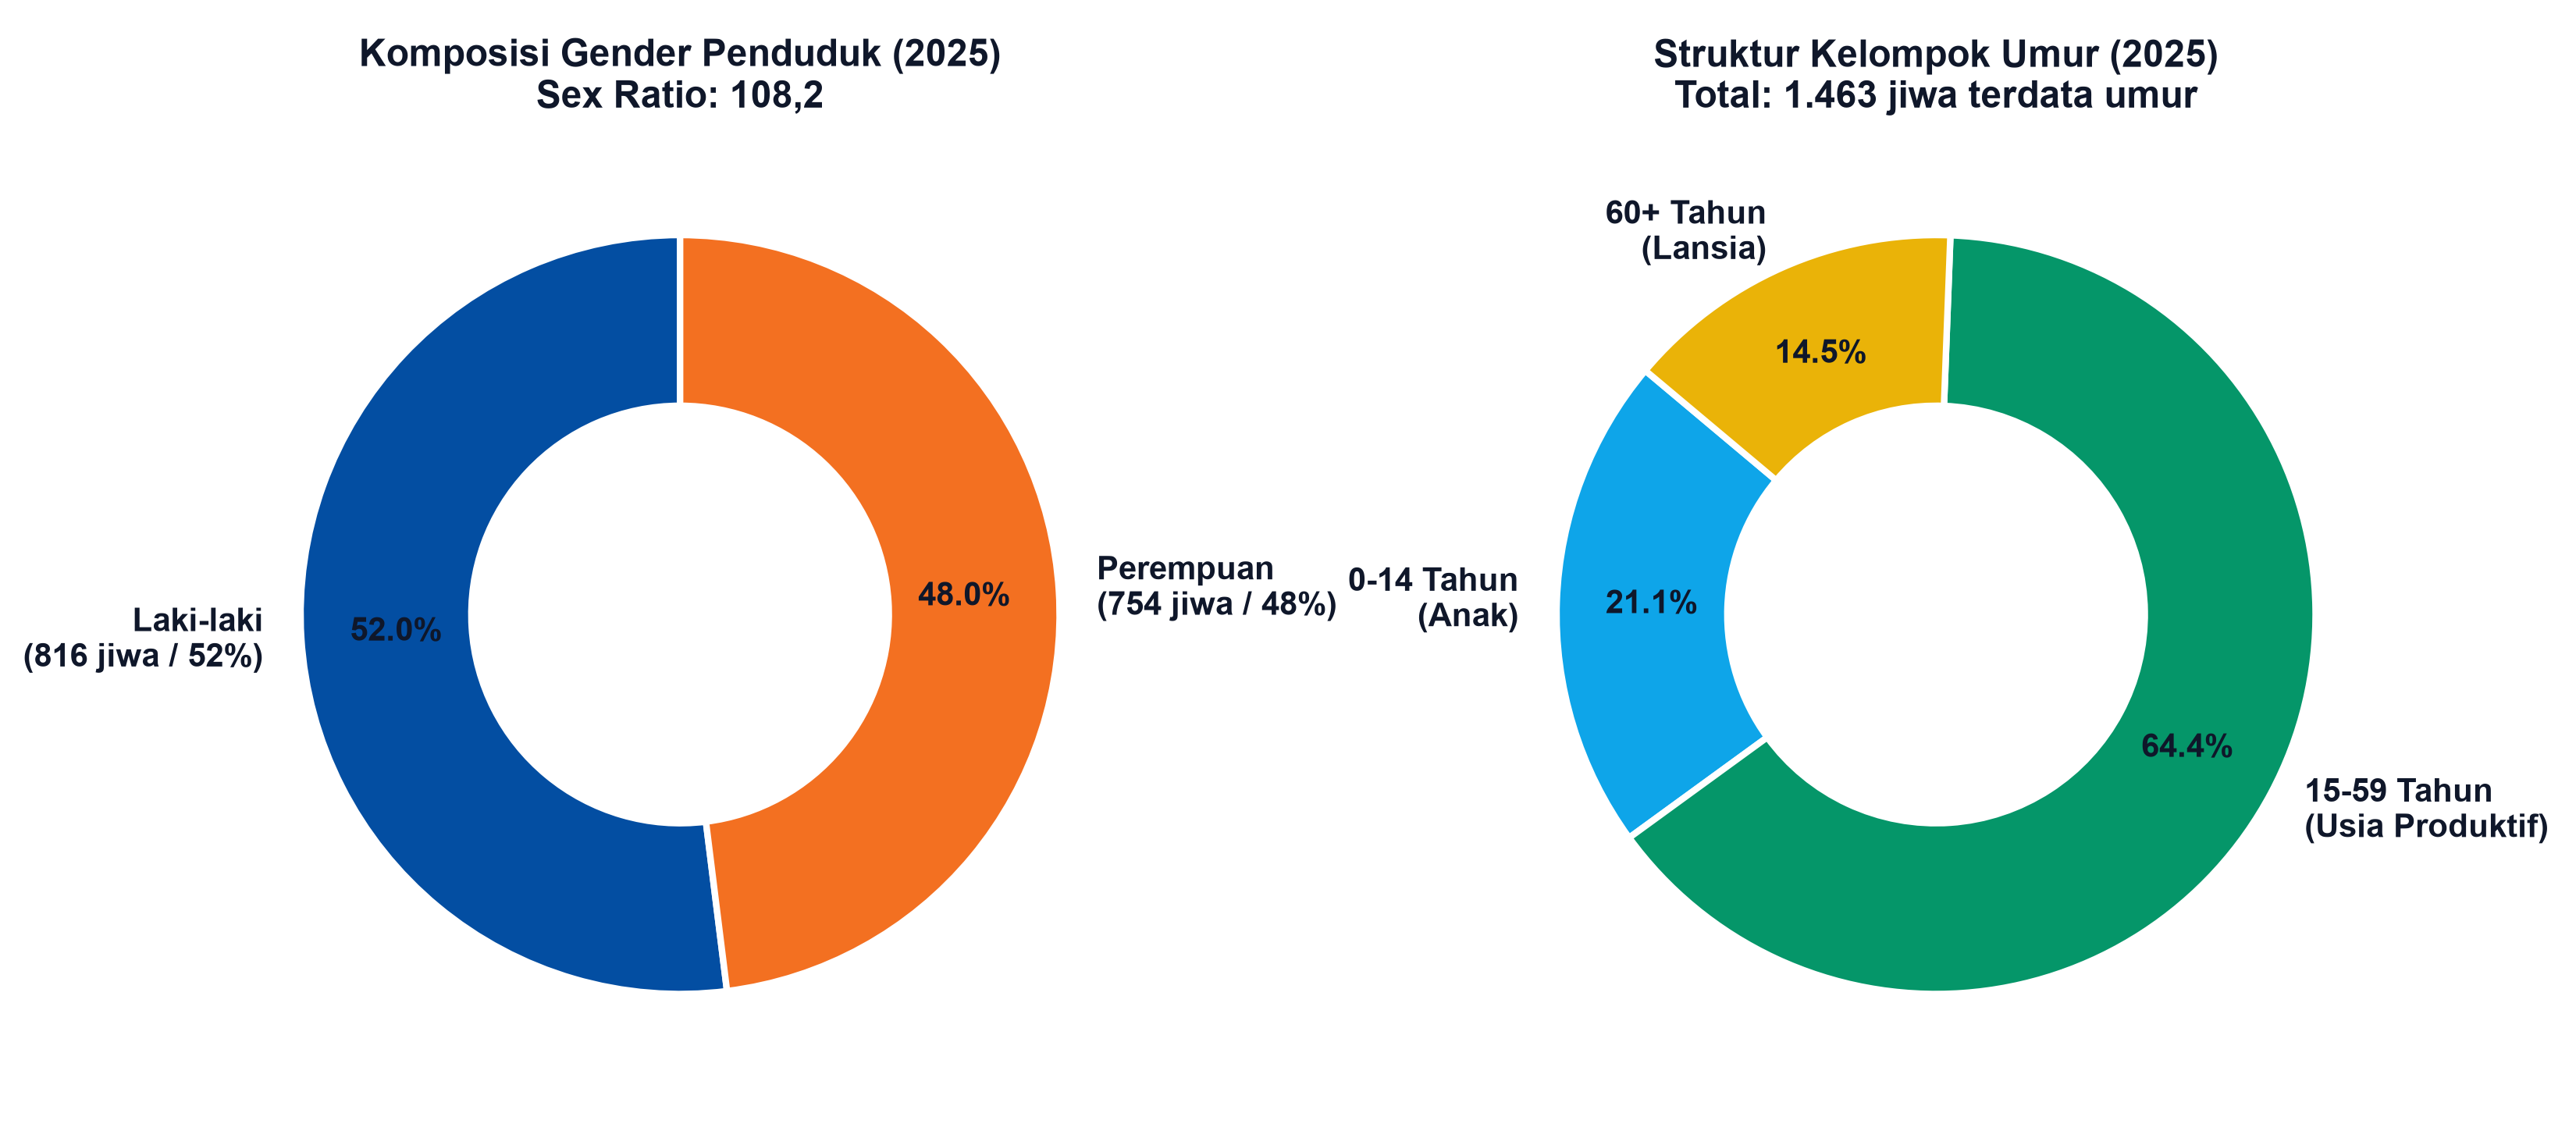
\includegraphics[width=0.88\textwidth]{images/grafik-3-struktur-umur.png}
  \caption{Komposisi Gender dan Struktur Kelompok Umur Penduduk (Tahun 2025)}
  \label{fig:grafik3}
\end{figure}

\noindent\small Komposisi gender relatif seimbang dengan \textit{Sex Ratio} 108,2 (816 laki-laki per 754 perempuan). Struktur umur menunjukkan dominasi kelompok usia produktif (15--59 tahun) yang mencapai \textbf{64,4\%} (942 jiwa), disusul usia anak-anak 0--14 tahun (21,1\%) dan kelompok lanjut usia 60+ tahun (14,5\%). Angka Rasio Ketergantungan (\textit{Dependency Ratio}) sebesar \textbf{55,3\%} menandakan kondisi bonus demografi aktif yang menjadi modal dasar pembangunan Desa Popontolen.

\vspace{0.4cm}

\begin{figure}[!htbp]
  \centering
  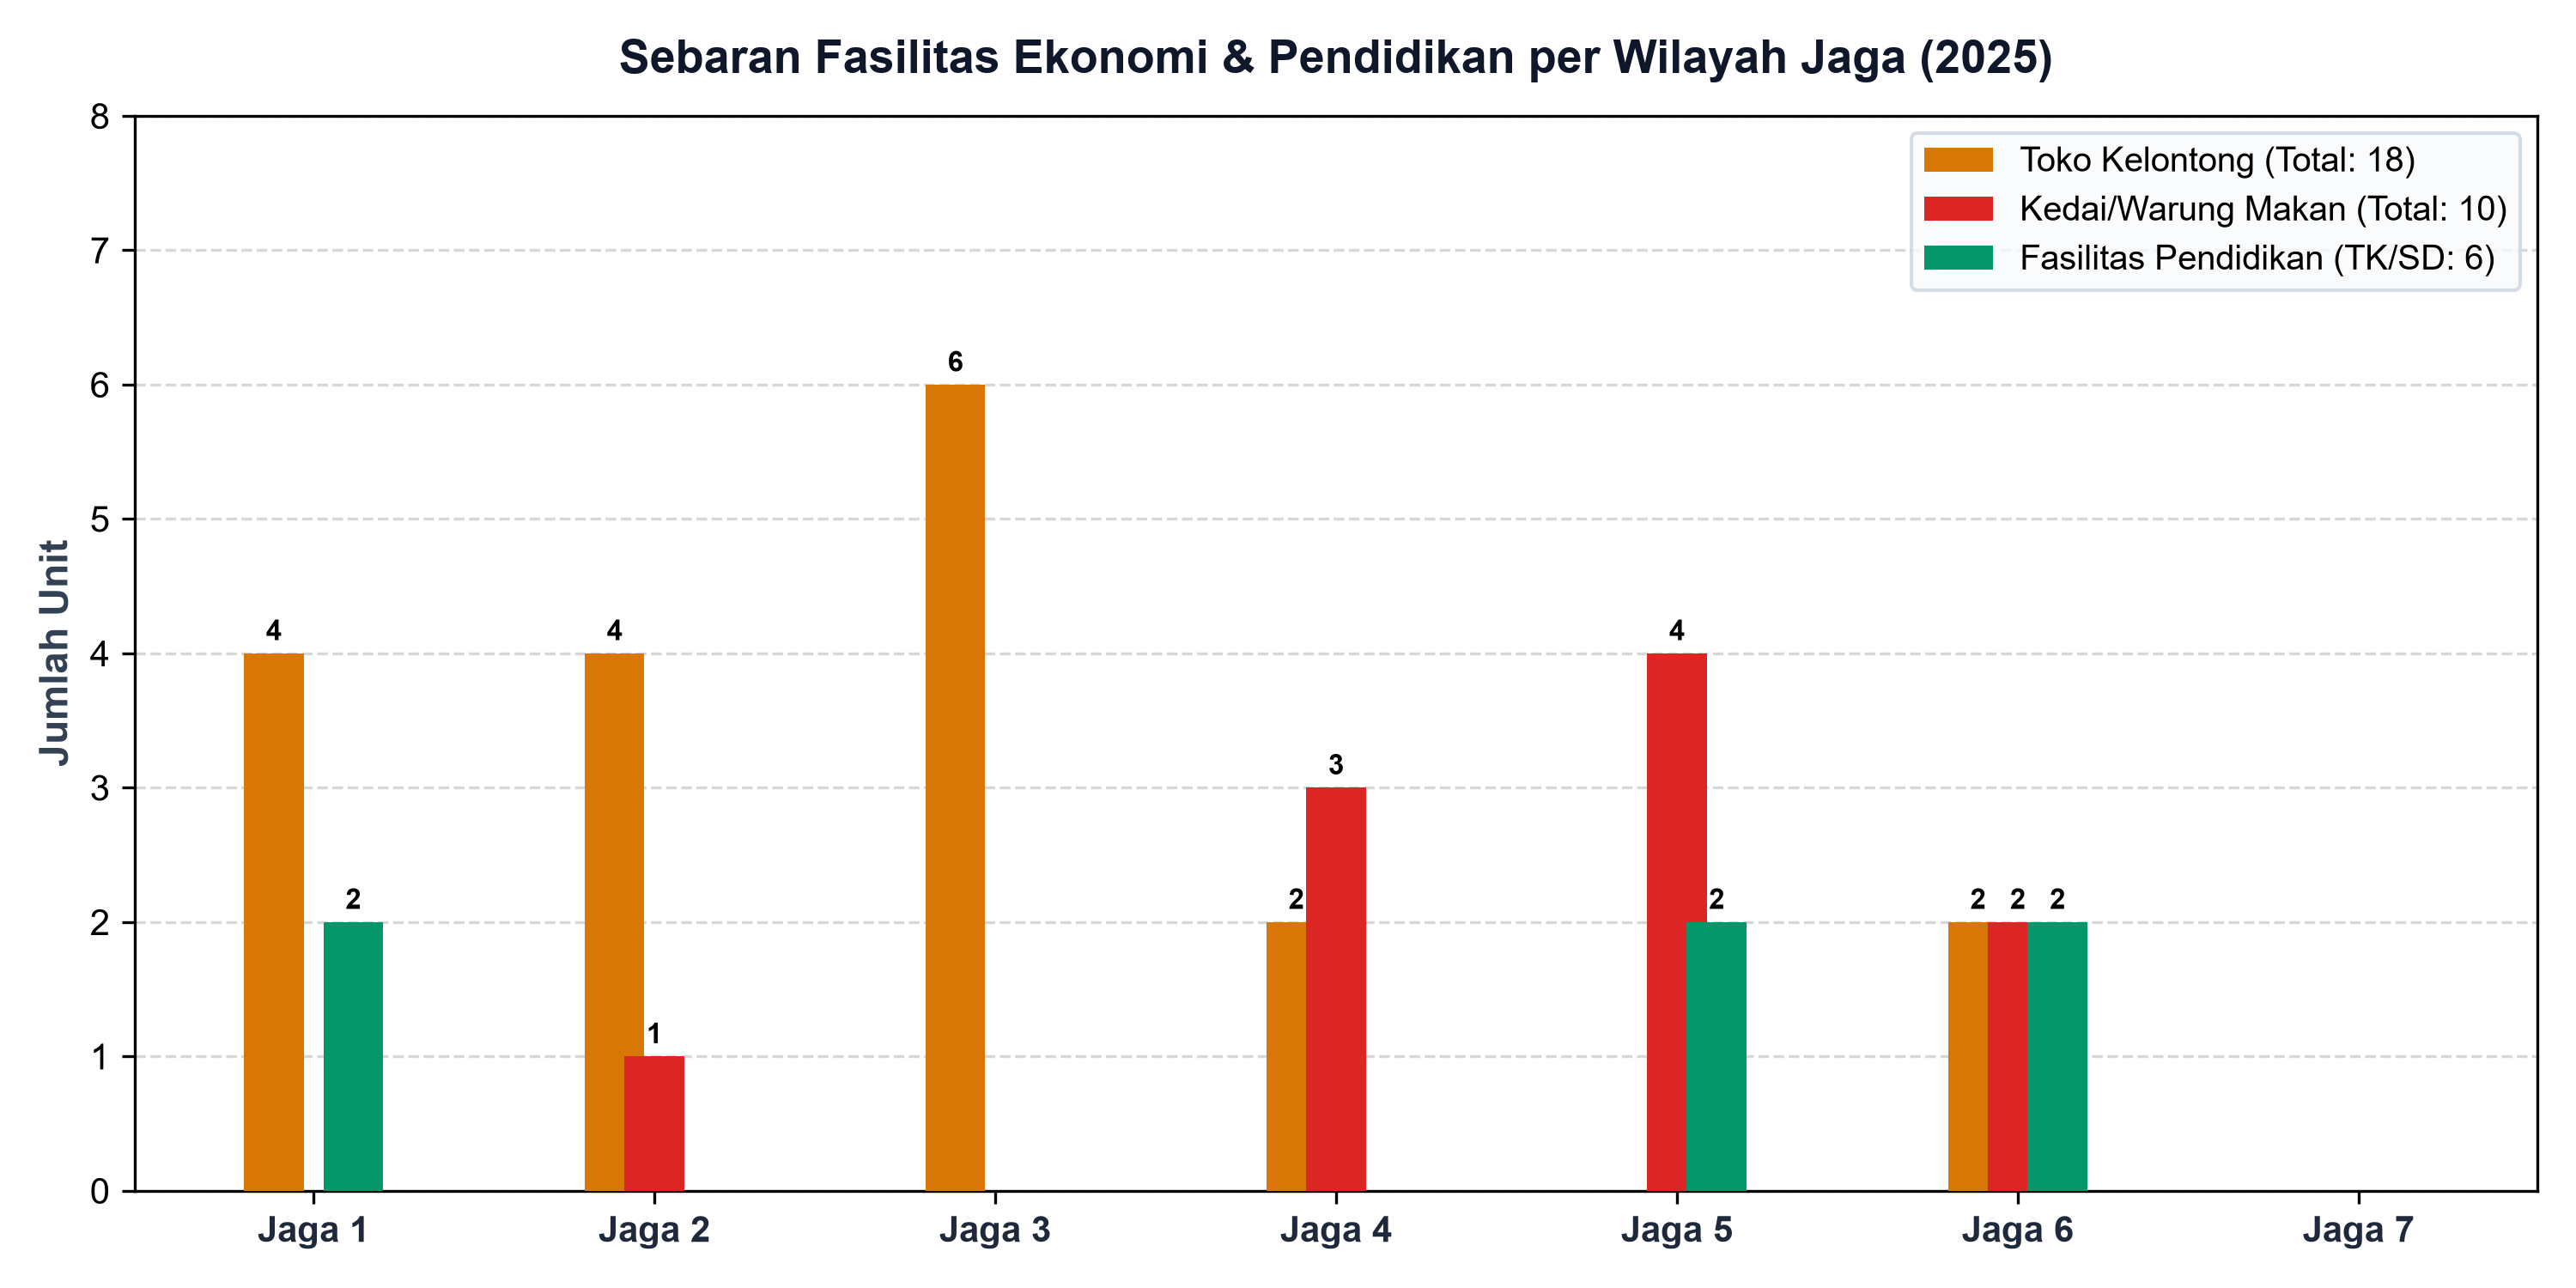
\includegraphics[width=0.85\textwidth]{images/grafik-4-fasilitas.png}
  \caption{Sebaran Fasilitas Ekonomi dan Sarana Pendidikan per Jaga (Tahun 2025)}
  \label{fig:grafik4}
\end{figure}

\noindent\small Fasilitas ekonomi mikro terkonsentrasi di \textbf{Jaga 2} (9 unit: 4 minimarket, 1 warung, 4 kelontong) dan \textbf{Jaga 3} (6 kelontong). Sebaliknya, \textbf{Jaga 7} sebagai wilayah terpadat belum memiliki fasilitas ekonomi formal. Sarana pendidikan dasar tersebar di 3 lokasi: Jaga 1 (TK Swasta + SD Negeri), Jaga 5 (TK Swasta + SD Negeri), dan Jaga 6 (TK Negeri + SD Negeri). Ketiadaan fasilitas SMP, SMA, dan perbankan menuntut penguatan konektivitas antarwilayah.
